\documentclass[12pt,hyperref,a4paper,UTF8]{ctexart}
\usepackage{HDUReport}
\usepackage{listings}
\usepackage{xcolor}
\usepackage{graphicx}
\usepackage{setspace}
\usepackage{float}
\setstretch{1.5} % 设置全局行距为1.5倍

\usepackage{enumitem} % 载入enumitem包以便自定义列表环境
\setlist[itemize]{itemsep=0pt, parsep=0pt} % 设置itemize环境的项目间距和段落间距

\setmainfont{Times New Roman} % 英文正文为Times New Roman


\usepackage{tikz}
\usetikzlibrary{shapes.geometric, arrows}
\usetikzlibrary{positioning, arrows.meta}
\usetikzlibrary{calc}
%封面页设置
{   
    %标题
    \title{ 
        \vspace{1cm}
        \heiti \Huge \textbf{《单片机原理及应用》作业报告} \par
        \vspace{1cm} 
        \heiti \Large {\underline{实验报告3第三部分:频率与占空比调节}   } 
        \vspace{3cm}
    
    }

    \author{
        \vspace{0.5cm}
        \kaishu\Large 学院\ \dlmu[9cm]{卓越学院} \\ %学院
        \vspace{0.5cm}
        \kaishu\Large 学号\ \dlmu[9cm]{23040447} \\ %班级
        \vspace{0.5cm}
        \kaishu\Large 姓名\ \dlmu[9cm]{陈文轩} \qquad  \\ %学号
        \vspace{0.5cm}
        \kaishu\Large 专业\ \dlmu[9cm]{智能硬件与系统(电子信息工程)} \qquad \\ %姓名 
    }
        
    \date{\today} % 默认为今天的日期,可以注释掉不显示日期
}
%%------------------------document环境开始------------------------%%
\begin{document}

%%-----------------------封面--------------------%%
\cover
\thispagestyle{empty} % 首页不显示页码
%%------------------摘要-------------%%
%\newpage
%\begin{abstract}




%\end{abstract}

%\thispagestyle{empty} % 首页不显示页码

%%--------------------------目录页------------------------%%
% \newpage
% \tableofcontents
% \thispagestyle{empty} % 目录不显示页码

%%------------------------正文页从这里开始-------------------%
\newpage
\setcounter{page}{1} % 让页码从正文开始编号

%%可选择这里也放一个标题
%\begin{center}
%    \title{ \Huge \textbf{{标题}}}
%\end{center}


\textbf{原题目:设计一个简易方波波形发生器,在按键K1(接INT0脚)的触发下可实现1KHz,100Hz,10Hz,1Hz的波形切换。用C语言编程。(选做:若按键K2(接INT1)实现当前频率波形下的占空比可调,如何实现?)}


\section{实验代码}

\begin{lstlisting}[language=C, caption={实验程序}]
#include <reg51.h>

// 宏定义
#define FOSC 12000000       // 晶振频率 12MHz
#define TIMER_RELOAD_1KHZ (65536 - FOSC / 12 / 2 / 1000 /2) // 1KHz定时器初值 因为是半周期
#define TIMER_RELOAD_100HZ (65536 - FOSC / 12 / 2 / 100 /2) // 100Hz定时器初值
#define TIMER_RELOAD_10HZ (65536 - FOSC / 12 / 2 / 10 /2)   // 10Hz定时器初值
//#define TIMER_RELOAD_1HZ (65536 - FOSC / 12 / 2 / 1 /2)     // 1Hz定时器初值 250,000超出范围了
//因为是半周期翻转电平 所以再乘以2补偿
sbit P2_0 = P2^0; // 方波输出引脚
unsigned char mode = 0; // 模式切换变量

// 外部中断1服务函数
void INT0_ISR(void) interrupt 0 {
    mode = (mode + 1) % 4; // 模式循环切换
}

// 定时器0中断服务函数
void Timer0_ISR(void) interrupt 1 {
        static int counter_1HZ=0; //基于10HZ的分频,计数十次就是1HZ
    TH0 = (mode == 0) ? (TIMER_RELOAD_1KHZ >> 8) :
            (mode == 1) ? (TIMER_RELOAD_100HZ >> 8) :
            (mode == 2) ? (TIMER_RELOAD_10HZ >> 8) :
                        (TIMER_RELOAD_10HZ >> 8);
    TL0 = (mode == 0) ? (TIMER_RELOAD_1KHZ & 0xFF) :
            (mode == 1) ? (TIMER_RELOAD_100HZ & 0xFF) :
            (mode == 2) ? (TIMER_RELOAD_10HZ & 0xFF) :
                        (TIMER_RELOAD_10HZ & 0xFF);
    
        if (mode==3) //1HZ
        {
            counter_1HZ++;
            if (counter_1HZ==10)
            {
                counter_1HZ=0;
                P2_0 = ~P2_0;
                
            }
        }
        else
        {
            P2_0 = ~P2_0; // 其他模式,直接翻转P2.0引脚电平
        }
    
}

void main() {
    // 初始化外部中断1
    IT0 = 1;  // 下降沿触发
    EX0 = 1;  // 使能外部中断0
    EA = 1;   // 开启总中断

    // 初始化定时器0
    TMOD = 0x01; // 定时器0,模式1(16位定时)
    TH0 = TIMER_RELOAD_1KHZ >> 8;
    TL0 = TIMER_RELOAD_1KHZ & 0xFF;
    ET0 = 1; // 使能定时器0中断
    TR0 = 1; // 启动定时器0

    P2_0 = 0; // 初始化P2.0为低电平

    while (1) {
        // 主循环,所有逻辑在中断中处理
    }
}
   
    
\end{lstlisting}

\section{实验效果}

\begin{figure}[H] % [H] 表示强制当前位置插入
    \centering
    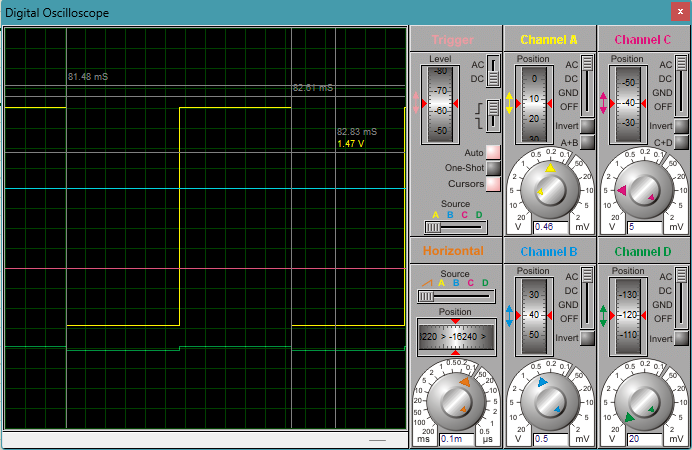
\includegraphics[width=0.9\textwidth]{figures/201.png} % 调整宽度为文本宽度的 80%
    \caption{Proteus示波器效果,1Khz方波 } %图片标题
    \label{fig:example} % 图片标签,用于引用
\end{figure}


\begin{figure}[H] % [H] 表示强制当前位置插入
    \centering
    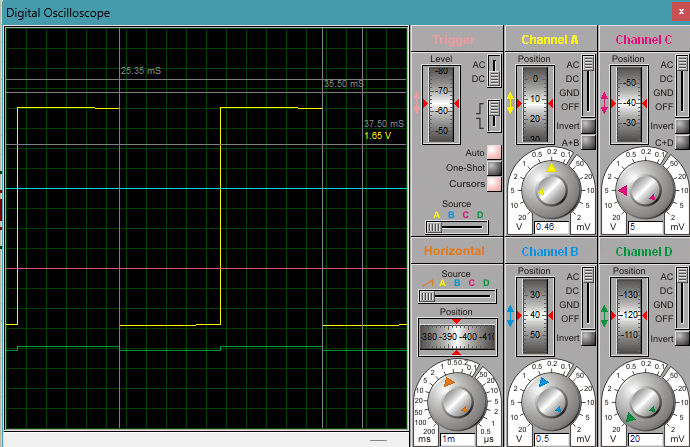
\includegraphics[width=1\textwidth]{figures/202.png} % 调整宽度为文本宽度的 80%
    \caption{Proteus示波器效果,100hz方波 } %图片标题
    \label{fig:example} % 图片标签,用于引用
\end{figure}


\begin{figure}[H] % [H] 表示强制当前位置插入
    \centering
    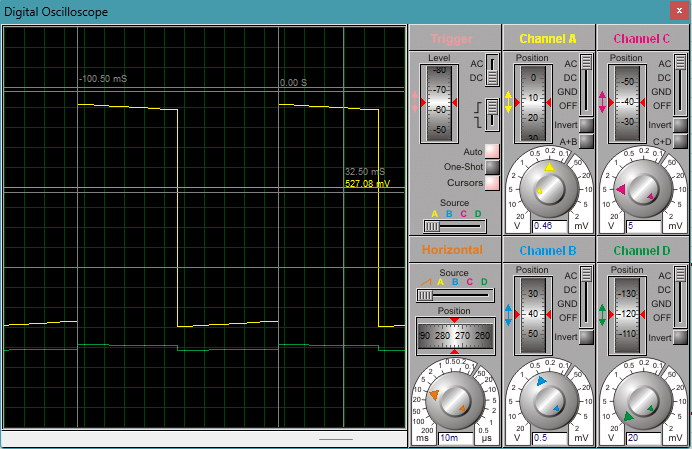
\includegraphics[width=1\textwidth]{figures/203.png} % 调整宽度为文本宽度的 80%
    \caption{Proteus示波器效果,10hz方波 } %图片标题
    \label{fig:example} % 图片标签,用于引用
\end{figure}


\begin{figure}[H] % [H] 表示强制当前位置插入
        \centering
        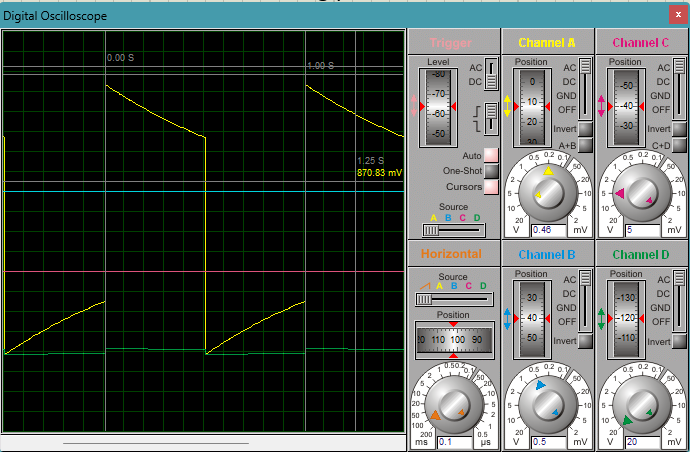
\includegraphics[width=1\textwidth]{figures/204.png} % 调整宽度为文本宽度的 80%
        \caption{Proteus示波器效果,1hz方波 } %图片标题
        \label{fig:example} % 图片标签,用于引用
\end{figure}


\begin{figure}[H] % [H] 表示强制当前位置插入
        \centering
        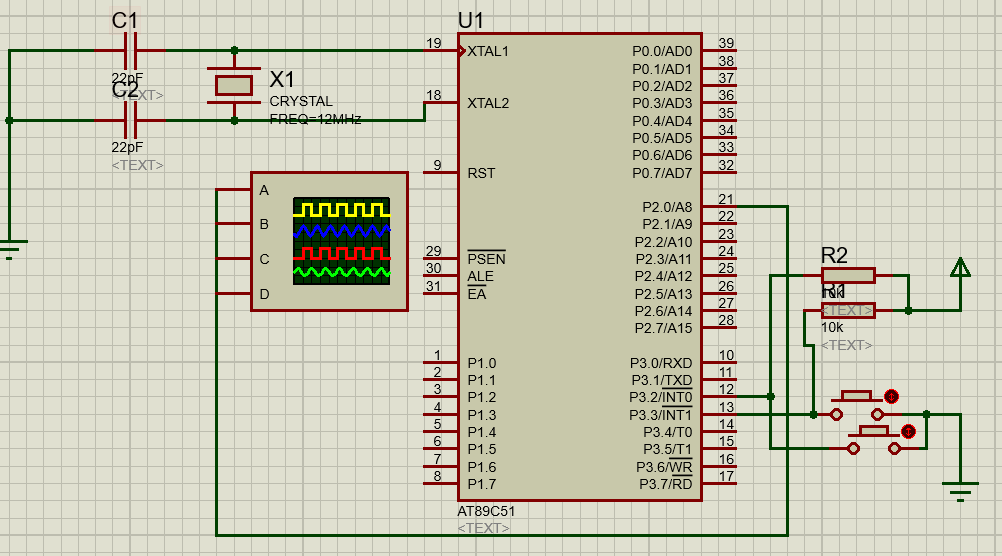
\includegraphics[width=0.9\textwidth]{figures/205.png} % 调整宽度为文本宽度的 80%
        \caption{Proteus电路结构 } %图片标题
        \label{fig:example} % 图片标签,用于引用
\end{figure}

\section{流程图}


\begin{figure}[H] % [H] 表示强制当前位置插入
        \centering
        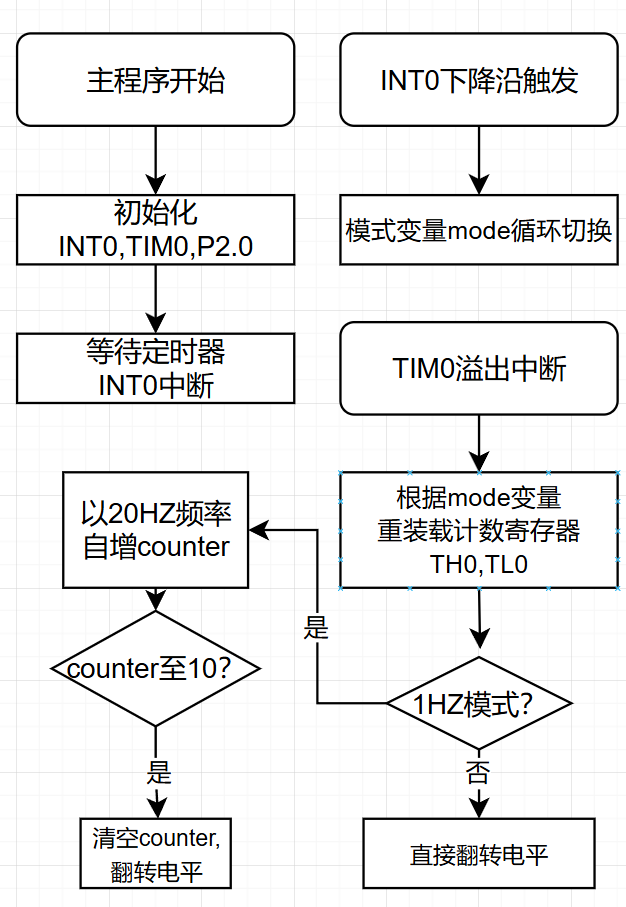
\includegraphics[width=0.9\textwidth]{figures/301.png} % 调整宽度为文本宽度的 80%
        \caption{系统控制流程图} %图片标题
        \label{fig:example} % 图片标签,用于引用
\end{figure}

\section{选做部分:占空比可调}

\subsection{实验代码}

\begin{lstlisting}[language=C, caption={实验程序}]
//拓展程序 占空比可调版本 可以调节10%至90%,步进10%
#include <reg51.h>

// 宏定义
#define FOSC 12000000       // 晶振频率 12MHz
#define TIMER_RELOAD_1KHZ (65536 - 1 ) // 1KHz定时器初值(半周期) 
//中断程序时间占用 影响频率较大 适当调参 但是周期是1.5ms左右
#define TIMER_RELOAD_100HZ (65536 - FOSC / 12 / 2 / 1000 ) // 100Hz定时器初值
#define TIMER_RELOAD_10HZ (65536 - FOSC / 12 / 2 / 100 )   // 10Hz定时器初值
//因为是半周期翻转电平 所以再除以2补偿

sbit P2_0 = P2^0; // 方波输出引脚
unsigned char mode = 0;       // 模式切换变量
unsigned char duty_cycle = 50; // 占空比,初始为50%

// 外部中断0服务函数(切换频率模式)
void INT0_ISR(void) interrupt 0 {
    mode = (mode + 1) % 4; // 模式循环切换
}

// 外部中断1服务函数(切换占空比)
void INT1_ISR(void) interrupt 2 {
    duty_cycle += 10; // 占空比增加10%
    if (duty_cycle > 90) {
        duty_cycle = 10; // 超过90%后回到10%
    }
}

// 定时器0中断服务函数
void Timer0_ISR(void) interrupt 1 {
    static unsigned int high_count = 0; // 高电平计数
    static unsigned int low_count = 0;  // 低电平计数
    static unsigned char state = 0;     // 当前状态:0为高电平,1为低电平
    static int counter_1HZ = 0;         // 基于10Hz的分频计数

    // 根据模式设置定时器初值
    unsigned int timer_reload = (mode == 0) ? TIMER_RELOAD_1KHZ :
                                (mode == 1) ? TIMER_RELOAD_100HZ :
                                (mode == 2) ? TIMER_RELOAD_10HZ :
                                                TIMER_RELOAD_10HZ; // 1Hz基于10Hz分频

    TH0 = timer_reload >> 8;
    TL0 = timer_reload & 0xFF;

    if (mode == 3) { // 1Hz模式
        counter_1HZ++;
        if (counter_1HZ == 10) { // 10Hz分频为1Hz
            counter_1HZ = 0;
            if (state == 0) { // 高电平状态
                high_count++;
                if (high_count >= duty_cycle / 10) { // 高电平持续时间达到占空比
                    high_count = 0;
                    state = 1; // 切换到低电平
                    P2_0 = 0;
                }
            } else { // 低电平状态
                low_count++;
                if (low_count >= (10 - duty_cycle / 10)) { // 低电平持续时间达到占空比
                    low_count = 0;
                    state = 0; // 切换到高电平
                    P2_0 = 1;
                }
            }
        }
    } else { // 其他模式
        if (state == 0) { // 高电平状态
            high_count++;
            if (high_count >= duty_cycle / 10) { // 高电平持续时间达到占空比
                high_count = 0;
                state = 1; // 切换到低电平
                P2_0 = 0;
            }
        } else { // 低电平状态
            low_count++;
            if (low_count >= (10 - duty_cycle / 10)) { // 低电平持续时间达到占空比
                low_count = 0;
                state = 0; // 切换到高电平
                P2_0 = 1;
            }
        }
    }
}

void main() {
    // 初始化外部中断0(切换频率模式)
    IT0 = 1;  // 下降沿触发
    EX0 = 1;  // 使能外部中断0

    // 初始化外部中断1(切换占空比)
    IT1 = 1;  // 下降沿触发
    EX1 = 1;  // 使能外部中断1

    // 初始化总中断
    EA = 1;   // 开启总中断

    // 初始化定时器0
    TMOD = 0x01; // 定时器0,模式1(16位定时)
    TH0 = TIMER_RELOAD_1KHZ >> 8;
    TL0 = TIMER_RELOAD_1KHZ & 0xFF;
    ET0 = 1; // 使能定时器0中断
    TR0 = 1; // 启动定时器0

    P2_0 = 0; // 初始化P2.0为低电平

    while (1) {
        // 主循环,所有逻辑在中断中处理
    }
}
    
    
\end{lstlisting}

此代码存在问题:1KHZ时频率不准,中断程序里面东西太多了,消耗了大量机器周期;1KHZ时无法调节占空比,其余都可以;其余频率都有一些误差,100HZ会略微偏小,还是中断程序里面东西太多的原因。


\subsection{实验效果}

\begin{figure}[H] % [H] 表示强制当前位置插入
        \centering
        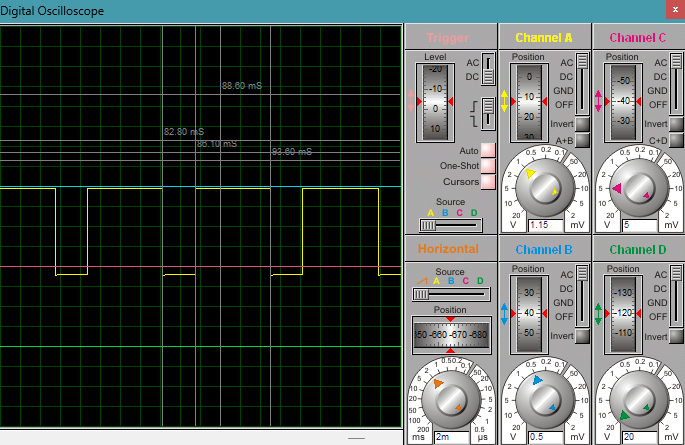
\includegraphics[width=0.9\textwidth]{figures/206.png} % 调整宽度为文本宽度的 80%
        \caption{100HZ,70\%占空比} %图片标题
        \label{fig:example} % 图片标签,用于引用
\end{figure}


\begin{figure}[H] % [H] 表示强制当前位置插入
        \centering
        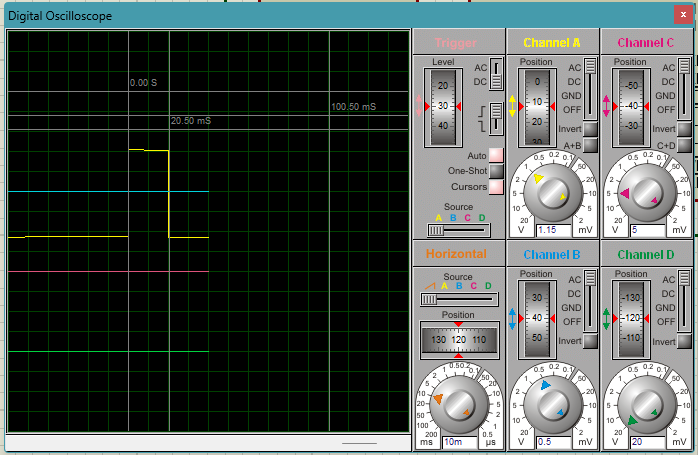
\includegraphics[width=0.9\textwidth]{figures/207.png} % 调整宽度为文本宽度的 80%
        \caption{10HZ,20\%占空比} %图片标题
        \label{fig:example} % 图片标签,用于引用
\end{figure}

\section{实验体会}


本次实验通过单片机定时器和中断的结合,实现了多频率方波的生成及占空比调节功能。实验过程中,发现1kHz频率下因中断程序复杂导致频率不准,优化中断代码是关键。此外,占空比调节功能在低频下表现较好,但高频时误差较大,需进一步优化定时器初值计算和中断处理效率。通过实验,初步理解了单片机定时器、中断机制及其对实时性的影响,提升了硬件编程能力。




\end{document}